%---------------------------------------------------------------------------------
%                西南交通大学研究生学位论文:第四章内容
%---------------------------------------------------------------------------------
\chapter{TCP/NC的改进及真实环境测试}
本章主要对文献\cite{Sundararajan2009}所提的TCP/NC给出几点改进,并加以实现,以验证相关性能。提出了前向重传机制以应对突发丢包;提出了一种新的自适应冗余度算法以应对网络的变化;对冗余包的发送时机给出改进以降低平均解码时延。
\section{前向重传机制}
通过冗余编码,TCP/NC可以很好地应对随机丢包网络的丢包。但当突发丢包发生时,TCP/NC表现就不好了。当突发丢包产生时,一般会要求重传,而TCP/NC的报文重传任务完全依赖TCP层。为了提高TCP/NC在突发丢包网络中的性能,本文提出了一种前向重传机制,能够同时高效地重传多个报文。
\par
通过增大TCP/NC的编码窗口可以提高TCP/NC应对突发丢包的能力,但是带来的后果是解码端运算复杂度的急剧增加,进而增大解码时延。在未发生超时重传时,TCP层是单个按序地重传各个丢失的报文的,因此TCP/NC会消耗很长一段时间来重传丢失的报文。图\ref{FR_EPS}展示了在丢了4个报文的情况下,TCP/NC是如何重传丢失的报文的。图\ref{FR_EPS}例子中设定的编码窗口值为2,冗余度为$\frac{1}{7}$,也就是说每7个编码包,多发一个冗余包。可以看到源端对$p_2$,$p_3$,$p_4$的重传总共耗费了3个RTT,导致目的端的NC层虽然在收到$C\left[8\right]$时就开始可以解码后面的报文,但无法将它们上交给上层的TCP。
\par
在标准TCP中,对于重复ACK采取的是快速重传的方法。以图\ref{FR_EPS}为例,源端的NC层在收到3个对$p_2$的ACK之后,直接将其交付给上层TCP。上层TCP收到3个重复的对$p_2$的ACK,认为报文$p_2$丢失了,采取快速重传,只重传$p_2$,然后继续接着$p_{10}$发送$p_{11}$。
\begin{figure}[htbp]
	\centering
	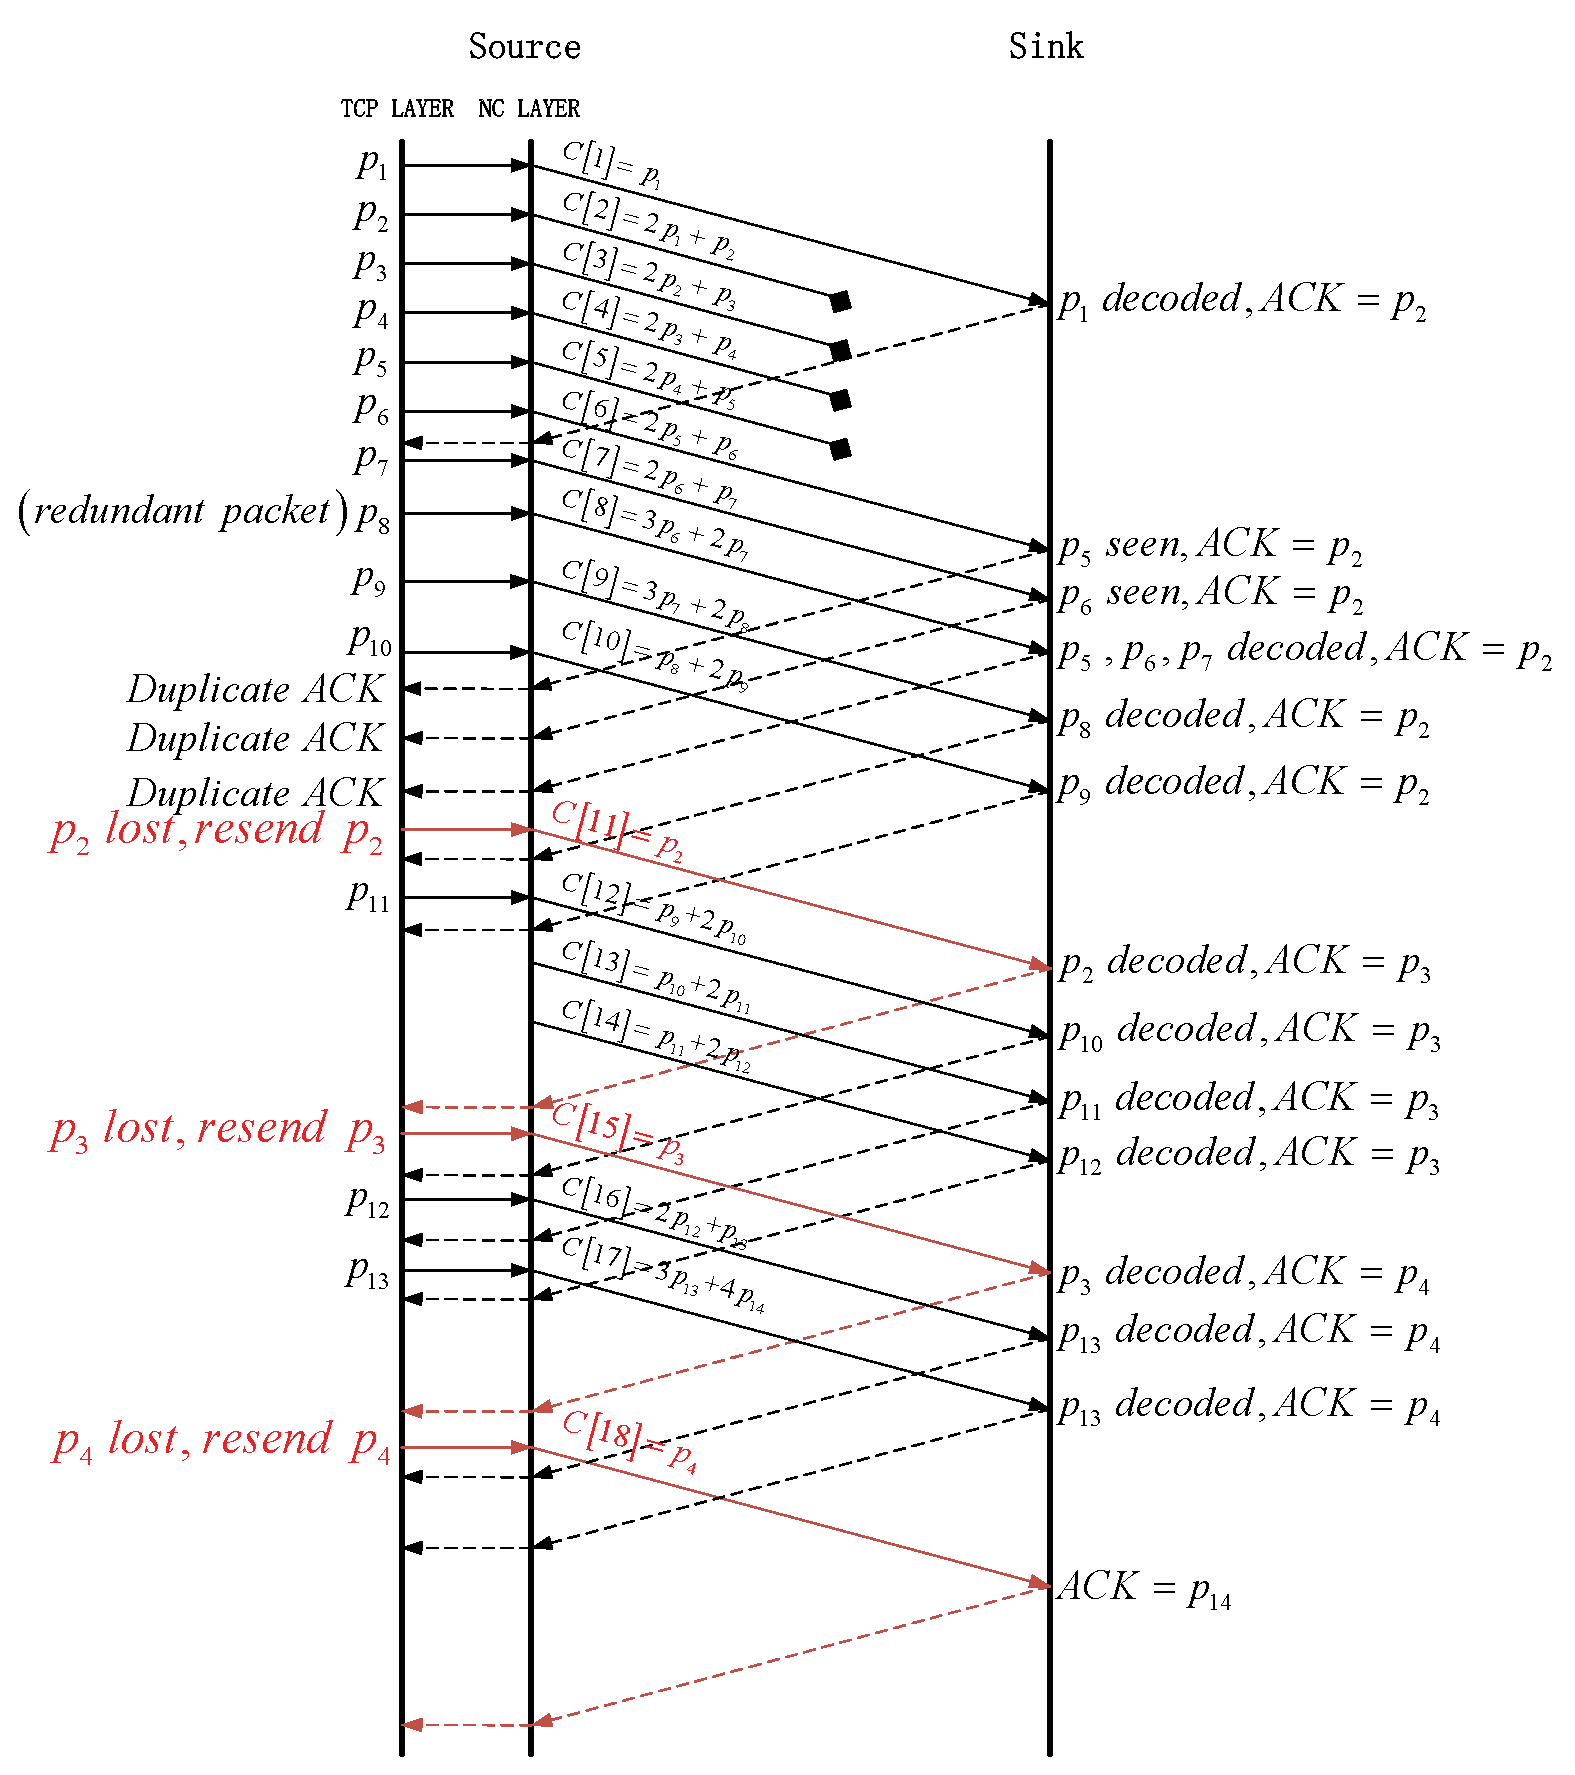
\includegraphics[width=4in]{figures/fr.eps}
	\caption{原有TCP/NC的重传机制}
	\label{FR_EPS}
\end{figure}
\subsection{无人机lossy信道环境搭建}
为了在真实丢包环境中测试TCP/NC及其改进协议的性能,本文搭建了无人机测试环境。将部署了TCP/NC改进协议的Raspberry Pi搭载在无人机上,通过WIFI无线链路来与地面站通信。 
\section{本章小结 }